\def \ti{\textit}
\def \bf{\textbf}

\chapter{Progettazione}
	\label{cap:progettazione}
	
    In questo capitolo verranno analizzate in dettaglio le scelte progettuali che hanno permesso la realizzazione del sistema software, considerando le limitazioni riscontrate nell'architettura del sistema stesso. Dopodiché si analizzerà, attraverso la rappresentazione dei diagrammi \textbf{UML}, la definizione delle fasi di sviluppo, ossia la progettazione delle funzionalità correnti dell'applicazione.

\section{Requisiti}
	\label{sec:requisiti}
	Come primo aspetto della progettazione si analizzeranno adesso i requisiti del sistema. Innanzitutto si deve specificare che l'intero sistema è pensato per essere utilizzato in un ambito amministrativo dove gli utenti possono essere per esempio i dipendenti di un'azienda. Questo vuol dire che ci si trova in un sistema chiuso in cui le persone che usano il sistema sono note. Tuttavia è possibile che nel tempo i dipendenti si licenzino oppure che ne sopraggiungano di nuovi, quindi deve essere presente una procedura che consenta di inserire nuovi utenti ed eventualmente di rimuovere quelli esistenti. In questo sistema dove gli utenti sono noti, immaginiamo la presenza di un utente \textbf{amministratore} che agisce come supervisore ed è l'unico ad avere la facoltà di abilitare gli utenti all'utilizzo del servizio nonché all'assegnazione del \emph{Trust~Level}.

Di seguito viene mostrato il diagramma dei casi d'uso che rappresenta una vista generale delle funzionalità del sistema.
	\begin{center}	
		\begin{figure}[H]
		\centering
		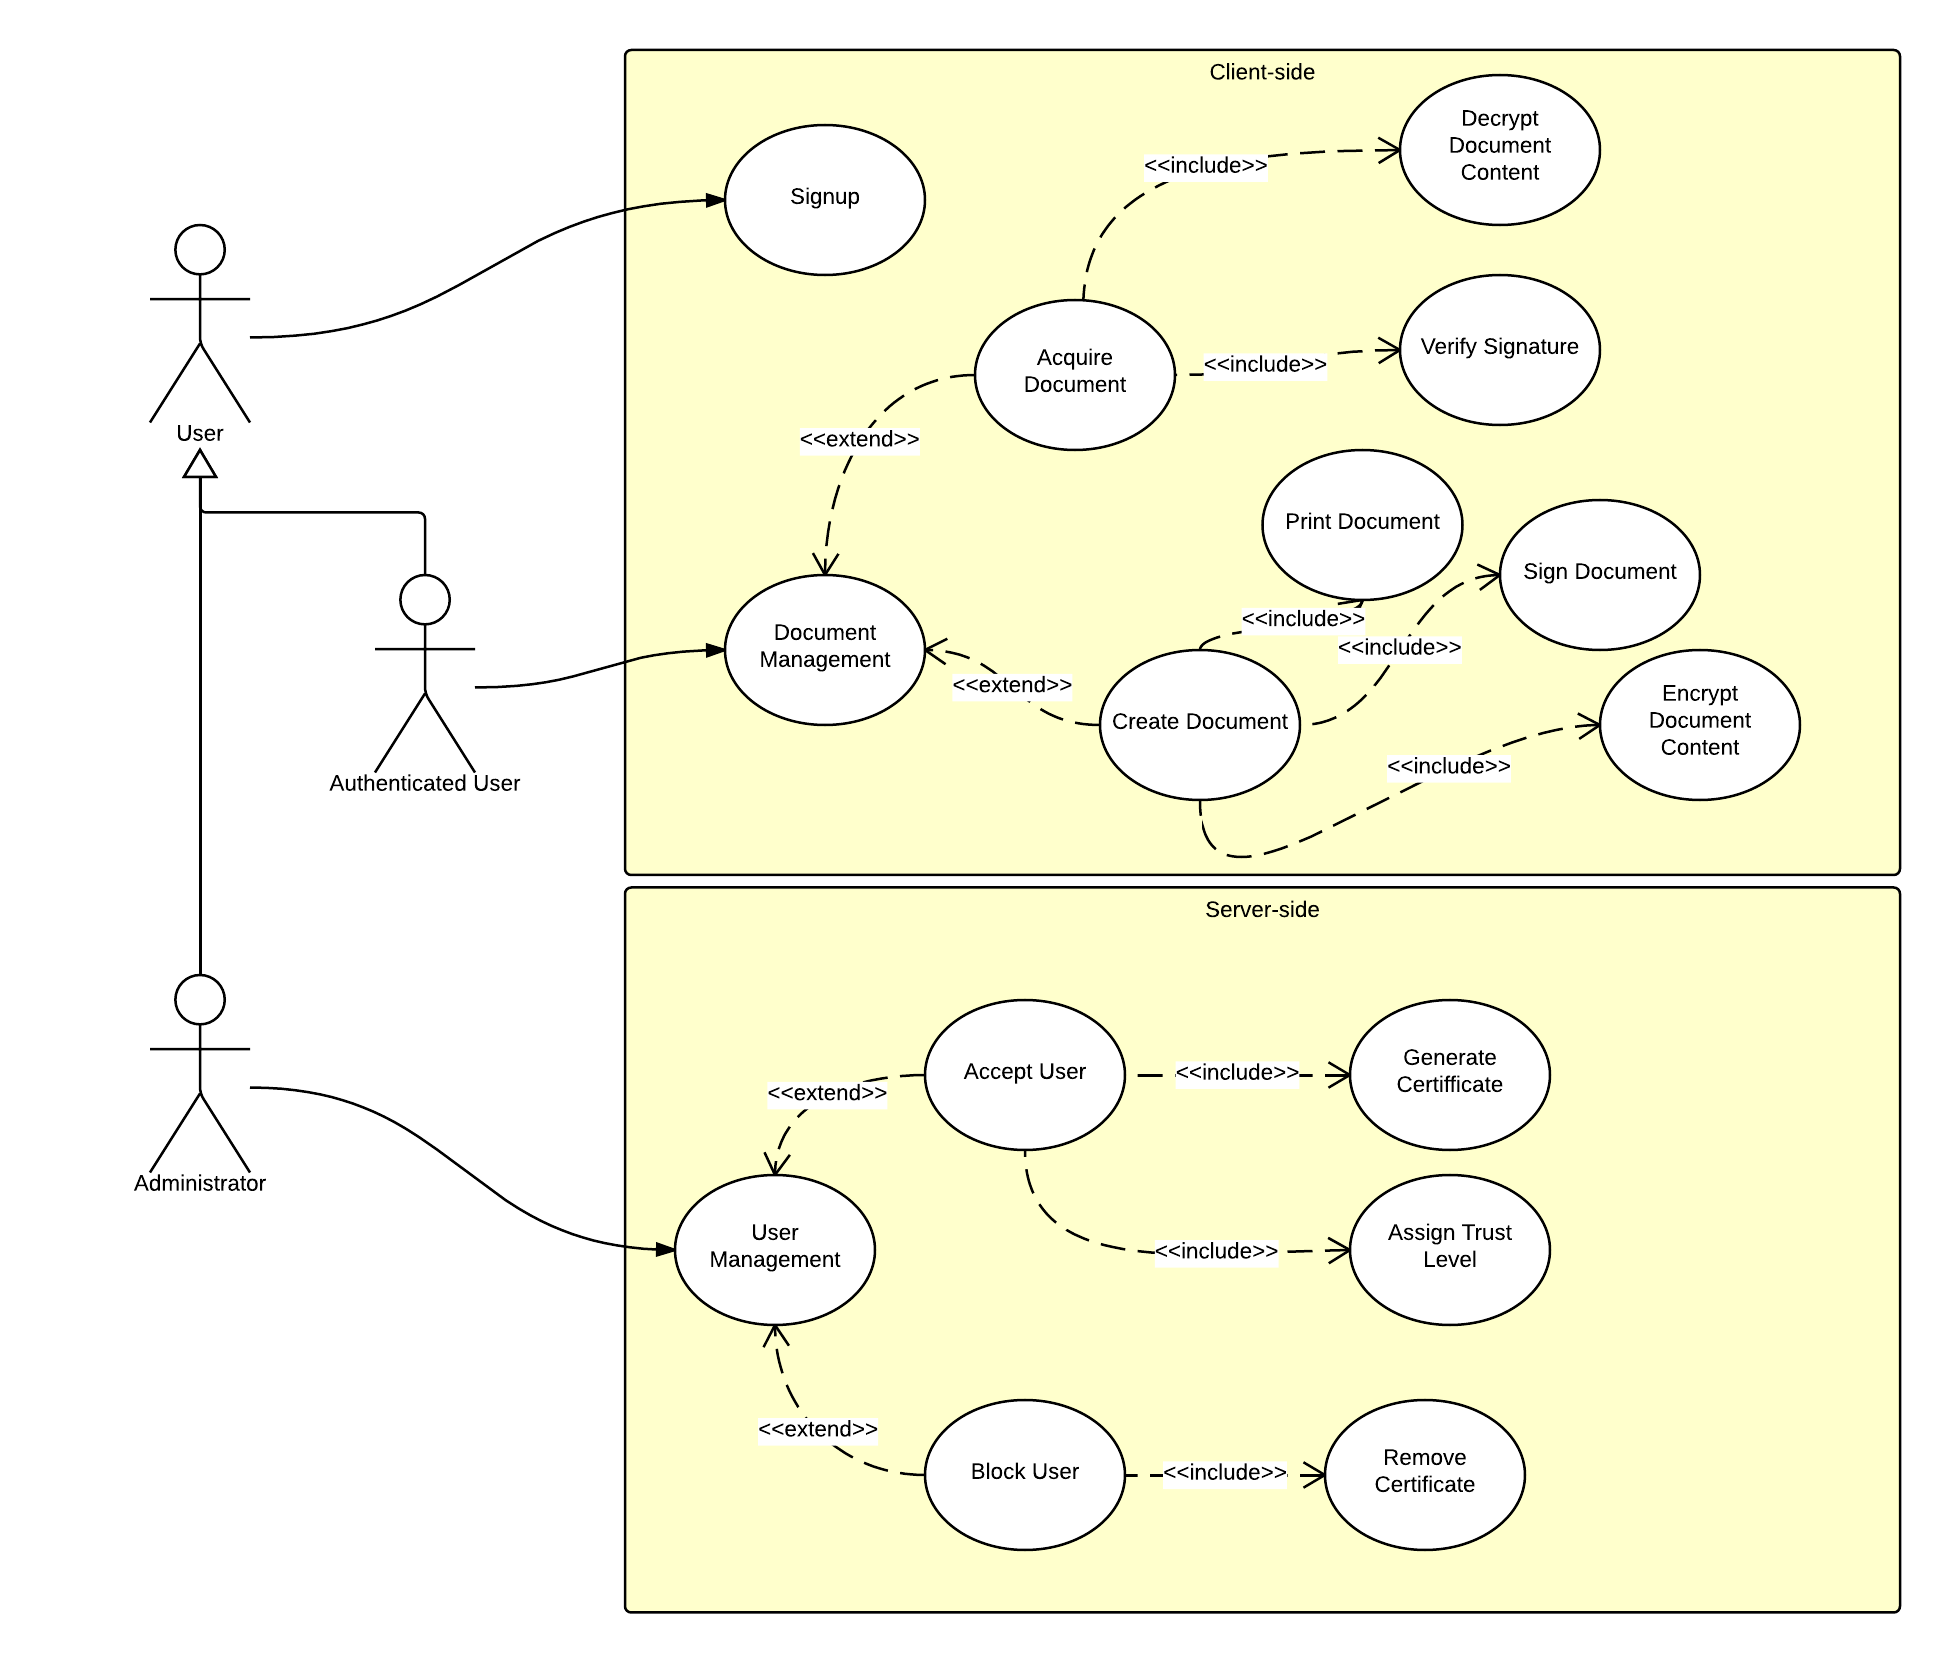
\includegraphics[scale=0.9]{Immagini/usecase}
		\caption[Use Case Diagram]{Diagramma dei casi d'uso del sistema software realizzato}
		\label{fig:usecase}
		\end{figure}
	\end{center}
La prima cosa che va evidenziata è che il tutto è strutturato secondo un architettura di tipo client/server. Questi due componenti dialogano tra di loro utilizzando una connessione sicura basata su SSL. Dettagli maggiori saranno dati nel paragrafo~\ref{sec:sicurezza}. Da quello che si può evincere, il server è un componente fondamentale che espone la funzionalità di \emph{provisioning} delle chiavi. Esso mantiene sia le chiavi di livello necessarie per la cifratura del documento, sia le chiavi pubbliche degli utenti registrati al sistema.

Da quello che si può vedere dalla figura~\ref{fig:usecase} nel sistema si hanno 3 attori importanti: l'amministratore, l'utente registrato (autenticato) e l'utente semplice che non ha mai utilizzato il sistema.
Come è stato già detto, l'amministratore si occupa 

\section{Architettura}
	\label{sec:architettura}
	%eventualmente diagrammi nel testo (senza capitolo dedicato)	
	
	%cosa fa client
	%cosa fa server
	%cenni al db: sqlite/mysql


\section{Gestione della sicurezza}
	\label{sec:sicurezza}
	%login - autenticazione forte
	%come si cripta: singolo/molti utenti
	%come si descripta
	%connessione al server
	%connessioni SSL - gestione certificati/keystore/mutua autenticazione	